\begin{figure}[h!]
	\begin{center}
		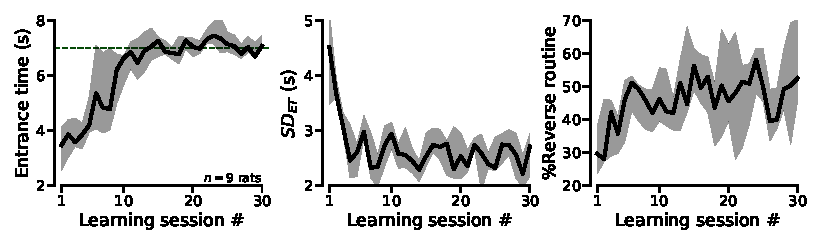
\includegraphics[scale=1]{ch-appendicies/figures/RevTrdLearning.pdf}
		\caption
		{\textbf{Performance improvement in the reverse treadmill task.}
		\textit{Left}: Entrance time across learning sessions.
		\textit{Middle}: Session-by-session standard deviation of ET.
		\textit{Right}: Percentage of trials during which animals used the run-and-wait (reverse) routine.
		}
		\label{fig:appendix:revLearn}
	\end{center}
\end{figure}